\documentclass[a4paper,12pt,final]{article} %Papierformat, Schriftgröße, BadBox markieren Bilder nich anzeigen (draft/final)
\usepackage[utf8]{inputenc}
\usepackage{lmodern,textcomp} %textfont deutlich runder/schöner + Eurozeichen richtig
%\renewcommand*\familydefault{\sfdefault} %Serifenlos
\usepackage[onehalfspacing]{setspace} %Zeilenabstand
\usepackage[left=2.6cm, right=2.6cm, top=3cm, bottom=3cm]{geometry} %Seitenränder
\usepackage{graphicx} %bilder (includegraphics)
\usepackage{todonotes}
\usepackage[hang]{footmisc} % Fußnoten 2. Zeile einrücken
\usepackage{float} %Positionierung von Bildern etc. [h] 
\usepackage{booktabs} %Tabellen
\usepackage{longtable}
\usepackage{amsmath}
\usepackage{multirow}
\usepackage{siunitx} %Zahlen zb exp oder einheiten
\usepackage{csquotes} %sonst bringt babble n Fehler
\usepackage[backend=biber, %Verarbeitet die BibTex datei und aktualisiert sich mit F11
			style=numeric-comp, %macht nummern aus den Quellen?!?
			sorting=none,]{biblatex} %stell sortiern nach Namen der Autoren aus
\DefineBibliographyStrings{ngerman}{ %macht aus u.a. -> et al.
   andothers = {{et\,al\adddot}}, 
}
\bibliography{Literatur.bib}  % Literatur verzeichniss
\usepackage[english,ngerman]{babel}  % The last language in the list is the primary one.
\usepackage{pdfpages} %zum Anhängen von PDF's
\usepackage[pdfusetitle, colorlinks, linkcolor=black, citecolor=black, urlcolor=gray,]{hyperref}  % Add clickable links for figures etc. Comment out for printing if desired.
\numberwithin{equation}{section} %nummeriert Formeln mit Kapitelnummer.Formelnummer ACHTUNG! muss nach hyperref kommen.
\numberwithin{figure}{section} %numeriert Bilder mit Kapitelnummer.Bildnummer ACHTUNG! muss nach hyperref kommen.
\numberwithin{table}{section} %numeriert Tabellen mit Kapitelnummer.Tabelle ACHTUNG! muss nach hyperref kommen.
\setcounter{biburllcpenalty}{9000}% Kleinbuchstaben?? mach die Zeilenumbrüche bei link's
\setcounter{biburlucpenalty}{9000}% Großbuchstaben?? mach die Zeilenumbrüche bei link's
\setcounter{tocdepth}{2} %Tiefe des Literaturverzeichnises, 2=inkl. subsecion so nur eine Seite Inhaltsverzeichnis
\setlength{\parindent}{0pt} %einrücken bei absätzen verhindern
\usepackage{listings}
\usepackage{color}

\definecolor{mygreen}{rgb}{0,0.6,0}
\definecolor{mygray}{rgb}{0.5,0.5,0.5}
\definecolor{mymauve}{rgb}{0.58,0,0.82}
\definecolor{bg_col}{rgb}{1,1,0.7}

\lstset{ %
  backgroundcolor=\color{bg_col},   % choose the background color
  basicstyle=\footnotesize,        % size of fonts used for the code
  breaklines=true,                 % automatic line breaking only at whitespace
  captionpos=b,                    % sets the caption-position to bottom
  commentstyle=\color{mygreen},    % comment style
  escapeinside={\%*}{*)},          % if you want to add LaTeX within your code
  keywordstyle=\color{blue},       % keyword style
  stringstyle=\color{mymauve},     % string literal style
}

\usepackage{fancyhdr} %Kopf/Fußzeile
\pagestyle{fancy}
\setlength{\headheight}{33.1pt}
%\setlength{\footheight}{30pt}
\lhead{\nouppercase{\leftmark}}
\rhead{
\includegraphics[width=2.5cm]{Bilder/logo.pdf}}
\lfoot{Abt \& Girke}
\cfoot{}
\rfoot{\thepage}
\renewcommand{\headrulewidth}{0.5pt}
\renewcommand{\footrulewidth}{0.5pt}

\begin{document}
\begin{center} %Titelseite
	\begin{figure}[h]
	\begin{center}
		
\includegraphics[width=8cm]{Bilder/logo.pdf} %bilder vertical anordnen zueinander
		\vspace{2cm}
	\end{center}
	\end{figure}
	\begin{Large}	
		\textbf{Entwicklung und Umsetzung einer intuitiven Steuerung für eine Roboterhand durch Erfassen
		der Geste einer menschlichen Hand\linebreak \linebreak Kinematik Labor\\}
		\vspace{1.5cm}
	\end{Large}
	\begin{large}
		des Studienganges Mechatronik und Robotik\linebreak		
		an der Frankfurt University of Applied Sciences\linebreak\linebreak
		von
		\begin{longtable}[b]{c c}
		Peter Abt & 1400337\\
		Felix Girke & 1386888\\
		\end{longtable}
		\vspace{1cm}
		\today\linebreak \linebreak
		\begin{longtable}[b]{p{7.9cm} p{6.9cm}}
		Bearbeitungszeitraum: & 9 Wochen\\
		Betreuer & Prof. Dr. Enno Wagner
		\end{longtable}
	\end{large}
\end{center} 
\thispagestyle{empty}%ende Titelseite
\setcounter{page}{0}
\newpage
\pagenumbering{Roman}
\markboth{Selbstständigkeitserklärung}{}
\section*{Selbstständigkeitserklärung}
\addcontentsline{toc}{section}{Selbstständigkeitserklärung} %Fügt das zum Inhaltsverzeichnis hinzu,
Wir versicheren hiermit, dass wir die Projektarbeit mit dem Thema: \glqq Entwicklung und Umsetzung einer intuitiven Steuerung für eine Roboterhand durch Erfassen
der Geste einer menschlichen Hand \grqq\ , selbst\-ständ\-ig verfasst und keine anderen als die angegebenen Quellen und Hilfsmittel benutzt haben.\vspace{2.5cm}
\begin{longtable}{p{5.5cm} p{3cm} p{6cm}}
 Frankfurt a. M., \today& & \\
 \cline{1-1} \cline{3-3}
 Ort, Datum& &Unterschrift (Abt)\\
\end{longtable}
\vspace{0.5cm}
\begin{longtable}{p{5.5cm} p{3cm} p{6cm}}
 Frankfurt a. M., \today& & \\
 \cline{1-1} \cline{3-3}
 Ort, Datum& &Unterschrift (Girke)\\
\end{longtable}
\addtocounter{table}{-1} % wird nicht mitgezählt bei der Tabellen Nr.
\newpage
%\markboth{Zusammenfassung}{}
%\section*{Zusammenfassung}
%\addcontentsline{toc}{section}{Zusammenfassung} %Fügt das zum Inhaltsverzeichnis hinzu
%\todo{brauchen wir das hier?}
%\newpage
\tableofcontents %Inhaltsverzeichis
\newpage
\phantomsection  %korregiert die links auf die Seite
\addcontentsline{toc}{section}{Abbildungsverzeichnis und Tabellenverzeichnis} %Fügt das Abbildungs zum Inhaltsverzeichnis hinzu
\listoffigures %abbildungsverzeichnis
\listoftables %tabellenverzeichnis
\newpage
\pagenumbering{arabic}
\section[Einleitung ]{Einleitung} \sectionmark{Einleitung}
Endeffektoren sind \glqq gewöhnlich das letzte Glied der kinematischen Kette einer Hand\-hab\-ungs\-ein\-richt\-ung\grqq\ \cite[S.302]{Hesse2013}. 
Schon früh wurde versucht mit Endeffektoren die men\-sch\-lich\-en Hand nachzubilden. Lange Zeit war diese Aufgabe zu komplex und es wurden Endeffektoren auf eine Aufgabe spezialisiert \cite[S.9]{VDI1990}.
Aber aufgrund der technischen Fortschritte der letzten Jahrzehnte gelingt es immer besser diese Komplexität zu be\-herr\-sch\-en.
So wurde 2013 mit der \glqq SVH 5-Finger-Hand\grqq\ die erste serienreife 5-Finger-Hand mit 9 Motoren von der Schunk GmbH \& Co. KG vorgestellt \cite[S.57]{Wolf2016}.
Durch die Arbeit vorheriger Gruppen, ist auch an der University of Applied Sciences in Frankfurt eine Roboterhand entwickelt und gebaut worden (Abbildung \ref{fig:RoboHand}), welche sich über einen Mikrocontroller steuern lässt.
\begin{figure}[H]
	\begin{center}
		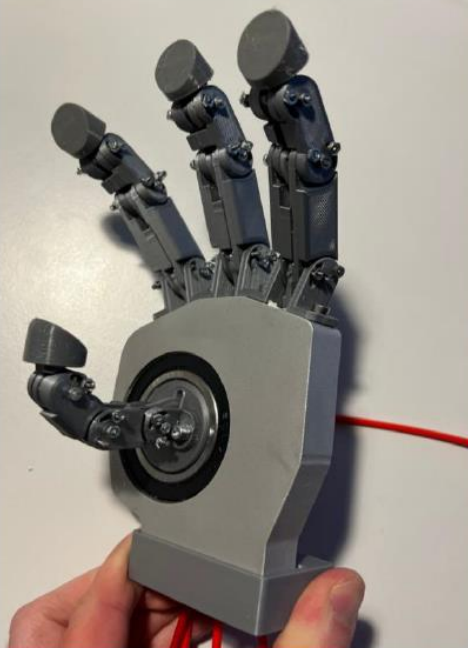
\includegraphics[height=8cm]{Bilder/RoboHandVorne.png}
		\vspace{0.5cm}
		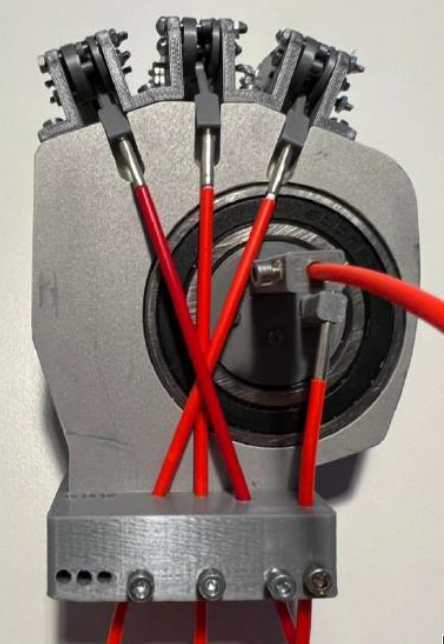
\includegraphics[height=8cm]{Bilder/RoboHandHinten.png}
		\caption{Die zu steuernde \glqq Frankfurter\grqq\ Roboter Hand}
		\label{fig:RoboHand}
	\end{center}
\end{figure}
Diese Roboterhand besteht aus drei Fingern und einem Daumen. Die einzelnen Finger werden über Bowdenzüge und Linearmotoren bewegt. Der Daumen kann rotieren, so dass ein Pinzettengriff mit jedem einzelnen der Finger möglich ist.
Die Ansteuerung geschieht über einen Arduino Mikrocontroller und vier verschiedene Knöpfe. Dies erfordert ein hohes Maß an Einarbeitung und Konzentration des Bedieners.
Deshalb wird versucht mit dieser Arbeit eine Ansteuerung zu schaffen welche intuitiver und einfacher ist. Hierzu soll versucht werden die Bewegung der Hand des Bedieners aufzuzeichnen und als Eingangssignal zu verwenden.
Besonderen Wert soll hierbei darauf gelegt werden die Vorteile der Hand, den Pinzettengriff, möglichst genau zu erreichen.
\newpage
\section{Stand der Technik}
\emph{Stand der Technik (Literatur/Patent-Recherche)}

Die Echtzeit-Erkennung von Handbewegungen ist für Steuerung von humanoiden Händen ist von Essenz. Die komplexen Bewegungsabläufe der menschlichen Hand lassen sich aufgrund der großen Anzahl an Fingersegmenten und Freiheitsgraden nur mit hohem Aufwand erfassen. Und eine Steuerung mittels Joysticks o.ä. ist ungeeignet.
Erste Versuche die Bewegungsabläufe der Hand aufzunehmen wurden mithilfe von in Handschuhen eingebauten Biegesensoren \cite{FlexSensor} und Lagesensoren durchgeführt.  Die zu dieser Zeit boomende Computerspielindustrie griff die Idee schnell auf und brachte den, technisch vereinfachten, PowerGlove \cite{PowerGlove} auf den Markt. Heute sind verschiedene Firmen im Markt die professionelle Systeme vertreiben wie CyberGlove Systems \cite{CyberGlove} oder Cobra Glove \cite{CobraGlove}. Diese bedienen sich meist der Erfassung der Fingerpositionen durch eine Kombination von mehreren an den Fingern angebrachten Inertial Measurment Units (IMUs) und Biegesensoren.

Handschuhe haben im allgemeinen einige Nachteile die sie mit sich bringen. Der an und Abziehvorgan ist umständlich, die Größe des Handschuhes muss stimmen, Desinfektionsmaßnahmen sind kompliziert.

Alternativ werden Handbewegungen auch mit Bewegungserkennungssystemen durch Marker und IR-Kamerasystemen aufgezeichnet. Über Triangolie die Position der einzellnen Markerpunkte berechnet. Hier ist die Firma VICON ein Vorreiter auf dem Markt.

Auch markerlose Kamerasysteme zur Bewegungserkennung existieren wie durch z.B. die Kinect Kamera ermöglicht.


\newpage
\section{Mögliche Konzepte}
\emph{Experimental (Vorgehen/Methoden zur Konstruktion, Berechnung, Simulation)}
Ziel ist es die Bewegungen der aufzunehmen.
Um eine ideale Lösung zu finden, werden verschiedene Lösungsmöglichkeiten skizziert und anschließend bewertet.
Wichtig für die Bewertung sind die Genauigkeit des Systems, die Flexibilität zwischen verschiedenen Anwendern und die entstehenden Kosten. 
\subsection{Bowdenzug über Finger}
Die komplexe, mehrdimensionale Bewegung der Finger kann über einen Bowdenzug abgegriffen werden und in eine lineare Bewegung verwandelt werden.
Inspiration hierzu ist die bestehende Roboter Hand (Abbildung \ref{fig:RoboHand}), welche die einzelnen Finger durch solche Bowdenzüge steuert.
Wird diese lineare Bewegung gemessen, so kann bestimmt werden wie stark ein Finger gekrümmt wird. 
\begin{figure}[H]
	\begin{center}
		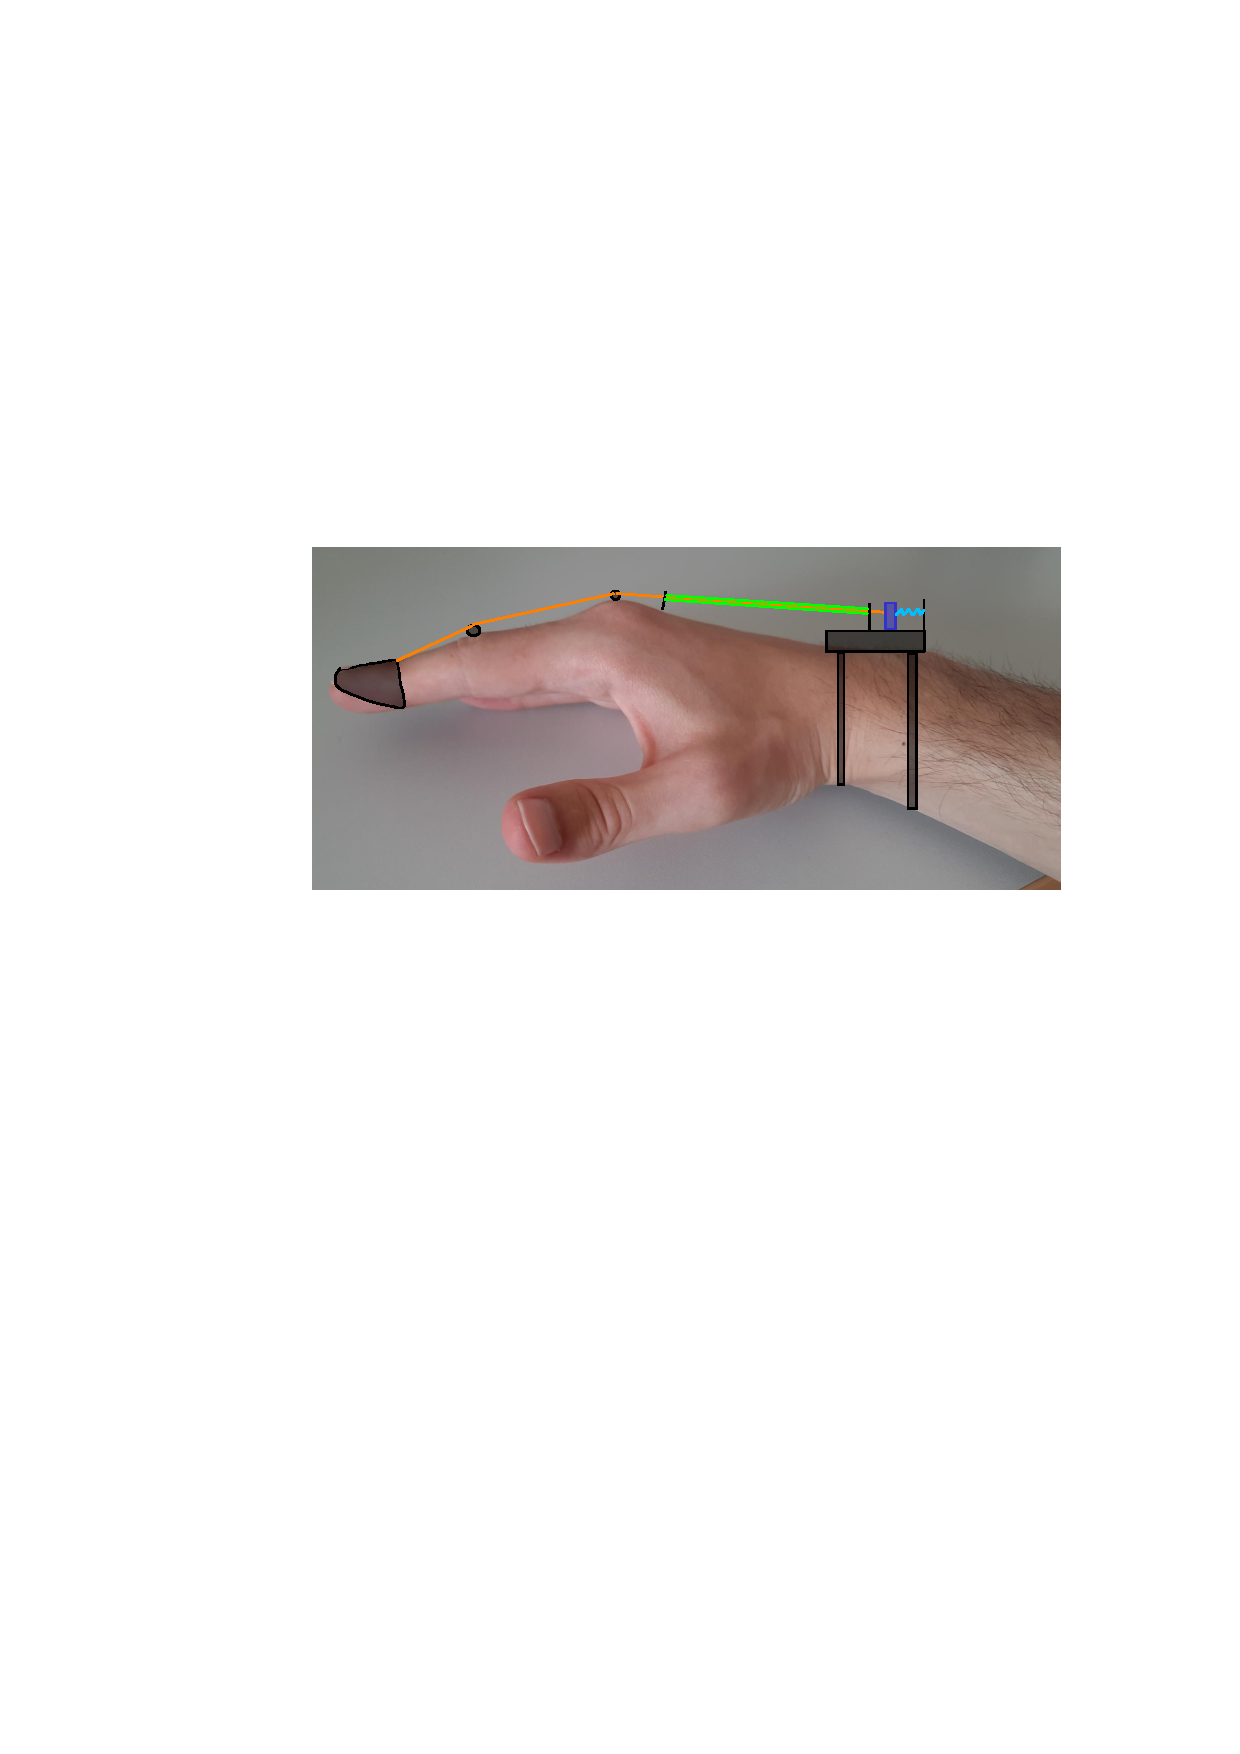
\includegraphics[width=10cm]{Bilder/HandPhoto1.pdf}
		\caption{Bautenzug über die Hand für die Finger}
		\label{fig:HandFinger}
	\end{center}
\end{figure}
In Abbildung \ref{fig:HandFinger} ist zu erkennen wie ein solcher Bowdenzug (orange) für die Finger angebracht werden könnte.
Das schwarze Objekte an der Fingerspitze ist der Befestigungspunkt des Bowdenzug, die schwarzen Kreise auf den Gelenken sind Führungen, damit der Bowdenzug nicht von den Fingern rutscht.
Hellgrün ist die Druckfeste Hülle des Bowdenzugs welche verhindert, dass die Bewegungen des Handgelenks in die Messung des Bowdenzugs eingeht.
Am rechten Ende des Bowdenzug befindet sich für jeden Finger ein lineares Potentiometer (dunkel Blau), welches von einer Feder in die Nullstellung zurückgezogen wird.
Es muss für jeden zu messenden Finger ein Potentiometer angebracht werden. Durch messen des Widerstandes des Potentiometers kann die Krümmung des Fingers in ein elektrisches Signal umgewandelt werden. Hierfür würde sich zum Beispiel ein Mikrocontroller eignen. 
Um die Punkte alle auf einer Hand zu befestigen eignet sich am Besten ein Handschuh. 
\begin{figure}[H]
	\begin{center}
		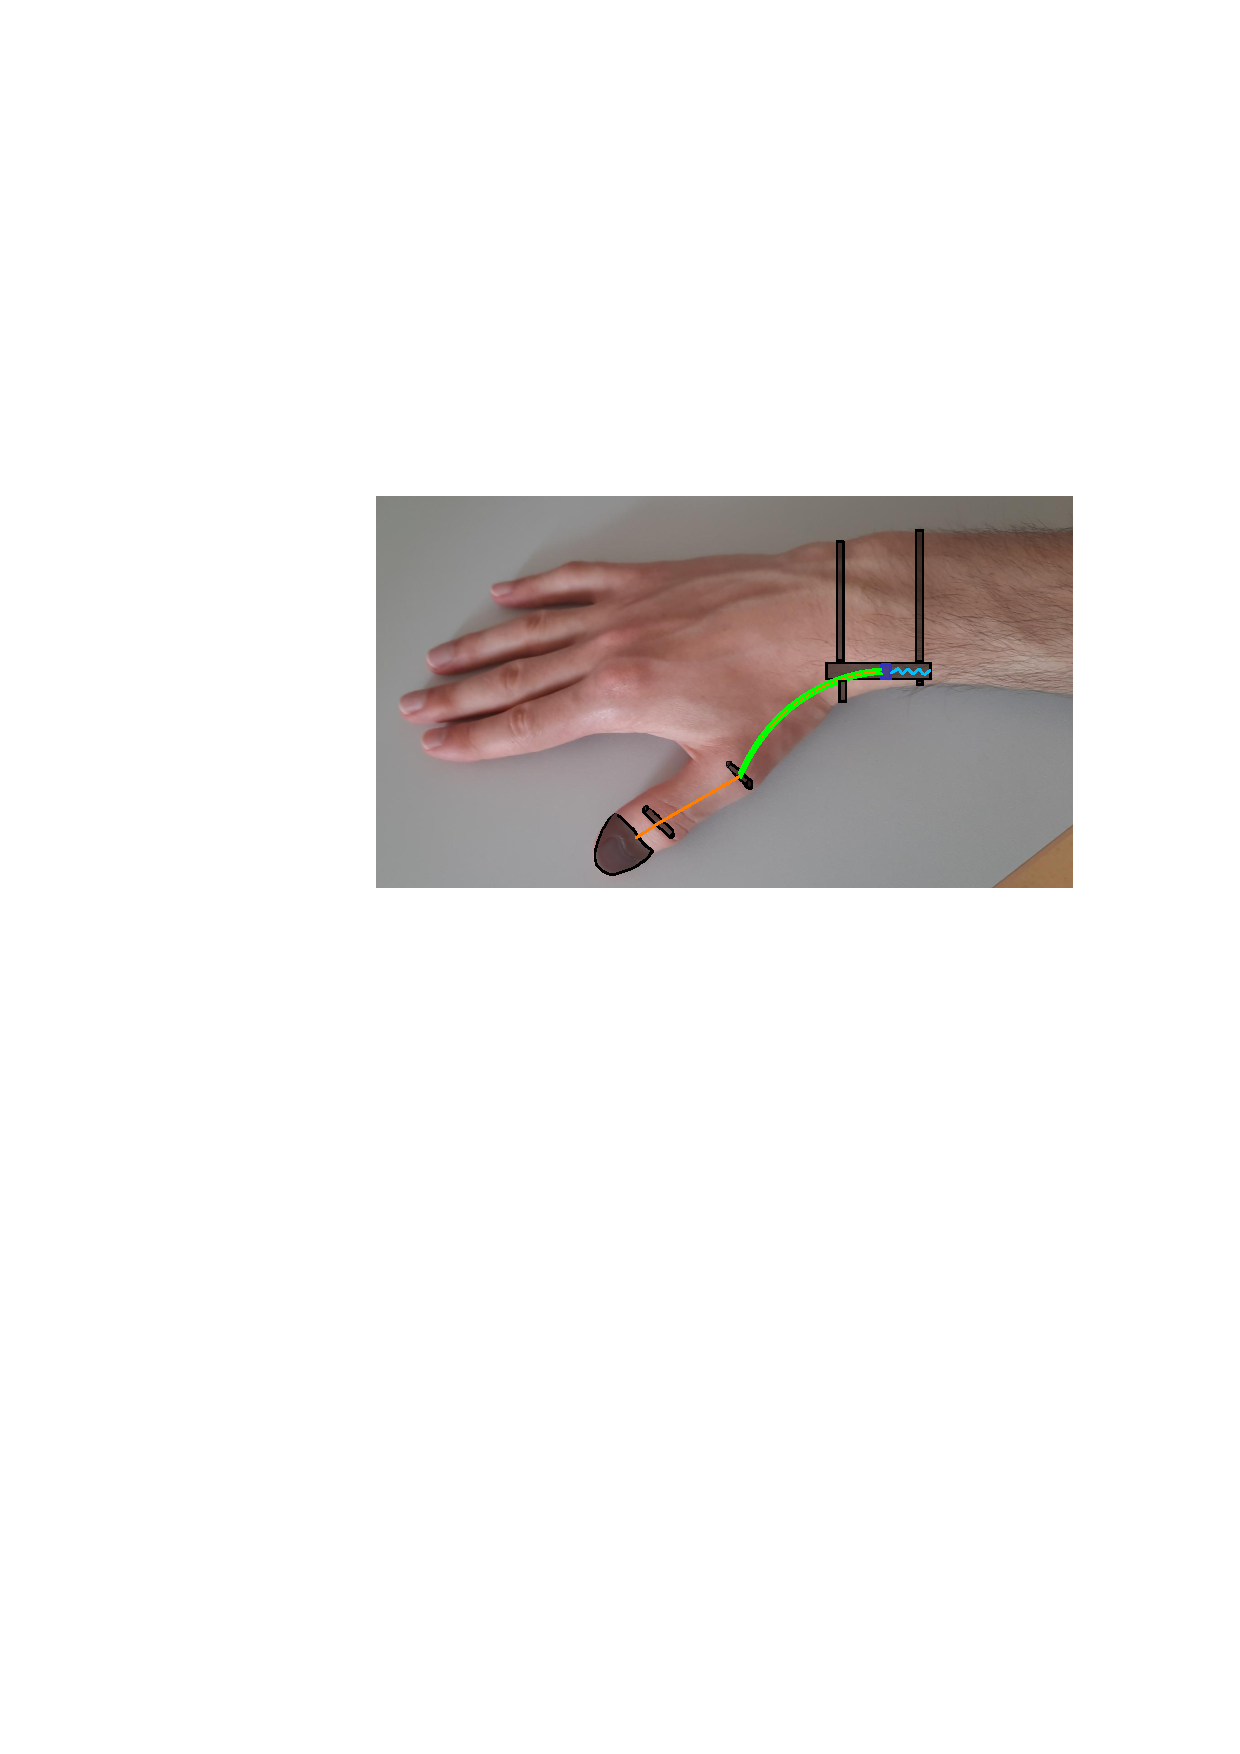
\includegraphics[width=10cm]{Bilder/HandPhoto2.pdf}
		\caption{Bautenzug über die Hand für den Daumen}
		\label{fig:HandDaumen}
	\end{center}
\end{figure}
Wird für die Messung des Daumens ähnlich vorgegangen (Abbildung \ref{fig:HandDaumen}), so werden die Messdaten wahrscheinlich wenig Aussagekraft haben.
Geht man mit dem Daumen die einzelnen Fingerspitzen des Pinzettengriffs durch so ist die Bewegung zwischen den einzelnen Fingerknochen sehr gering. Die Bewegung findet lediglich zwischen den Hand\-wur\-zel\-knoch\-en und dem ersten Fingerknochen statt.
Diese Bewegung liegt direkt neben der Bewegung des Handgelenks und ist schwieriger voneinander zu trennen. Des Weiteren ist die Bewegung des Daumens beim Pinzettengriff nur sehr gering weshalb  die Unterscheidung zu welcher Fingerspitze der Daumen sich bewegt schwer ist.\\
Sind alle Bowdenzüge perfekt angebracht, so ist es theoretisch möglich in einer zukünftigen Arbeit einen Servomotor parallel zu den Potentiometer anzubringen und somit die Bowdenzüge zu spannen.
Hierdurch könnte dem Nutzer simuliert werden, es würde sich ein Gegenstand zwischen den Fingern befinden, da eine Kraft auf die sich schließenden Finger ausgewirkt werden kann.  
\subsection{Biegesensoren DMS}
Die heutzutage erhältlichen Biegesensoren sind wesenlicht preiswerter als die ersten ihrer Art. Sie basieren nicht mehr auf dem Prinzip eines Lichwellenleiters sondern auf der Änderung der Leitfähigkeit von Materialien durch deren Biegung. Somit ermöglichen sie eine Einfache Möglichkeit den Gebogenheitsgrad eines einzellnen Fingers zu bestimmen. Als schwieriger erweißt sich jedoch die Positionsbestimmung des Daumens. Dieser kann sich auch unabhängig seines Biegegrades auf dem unteren Sattelgelenk in zwei Freiheitsgraden bewegen. Ein Begesensor reicht nicht um z.B. den Pinzettengriff zwischen Daumen und Zeigefinger und zwischen Daumen und Mittelfinger zu unterschieden.

\subsection{Image Processing}
Mithilfe des Einsatzes von moderner Bildverarbeitung und künstlicher Intelligenz lassen sich viele Probleme der vorherigen Methoden vermeiden. So sind allen vorran die benötigten Investitionen nahe Null. Lediglich ein PC sowei eine passende Webcam sind bereits aussreichen um die Positionserkennung zu ermöglichen. Ausserdem fallen umständliches an und abziehen eines sensiblne Handschuhes so wie der damit verbundene verkabelungs Aufwand weg.
\subsection{Entscheidung}
Bowdenzug negativ handschuh größe, Handschuh verrutscht leicht, Daumen kaum/ nicht messbar, (aufwendig), 
\newpage
\section{Umsetzung des Konzepts}
\emph{Ergebnisse (CAD-Modelle, Funktionsmuster, Messdaten, etc.)}\\
\subsection{HTTP code}
\subsection{LabVIEW}
Für die Roboterhand wird derzeit eine Steuerung in LabVIEW von einem anderen Team entwickelt. 
Deshalb müssen die erfassten Daten nach LabVIEW übertragen werden. Hierfür wird mit LabVIEW ein lokaler Server Programmiert, welcher von der Weboberfläche per GET-Request angesprochen wird und die entsprechenden Daten übertragen bekommt \cite{NIwebserverTutorial}.
Das angelegte LabVIEW Projekt besteht aus dem WebServerHand und den \\SharedVariables.lvlib (Abbildung \ref{fig:ProjektExplorer}).
\begin{figure}[H]
	\begin{center}
		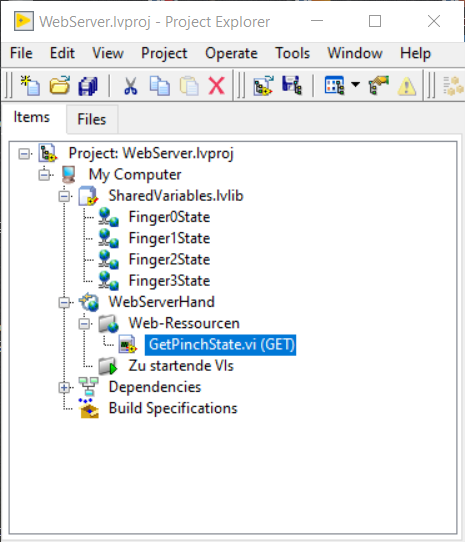
\includegraphics[width=7cm]{Bilder/ProjektExplorer.png}
		\caption{Übersicht der Dateien des LabVIEW Projektes}
		\label{fig:ProjektExplorer}
	\end{center}
\end{figure}
In dem Server ist eine GET-Methode angelegt namens GetPinchState.vi. Diese besteht aus einem User Panel (Abbildung \ref{fig:LabVIEWuserPanel}), einem Block Diagram (Abbildung \ref{fig:LabVIEWBlockDia}) und einem Connector Pane (Abbildung \ref{fig:LabVIEWConnectorPane}).
\begin{figure}[H]
	\begin{center}
		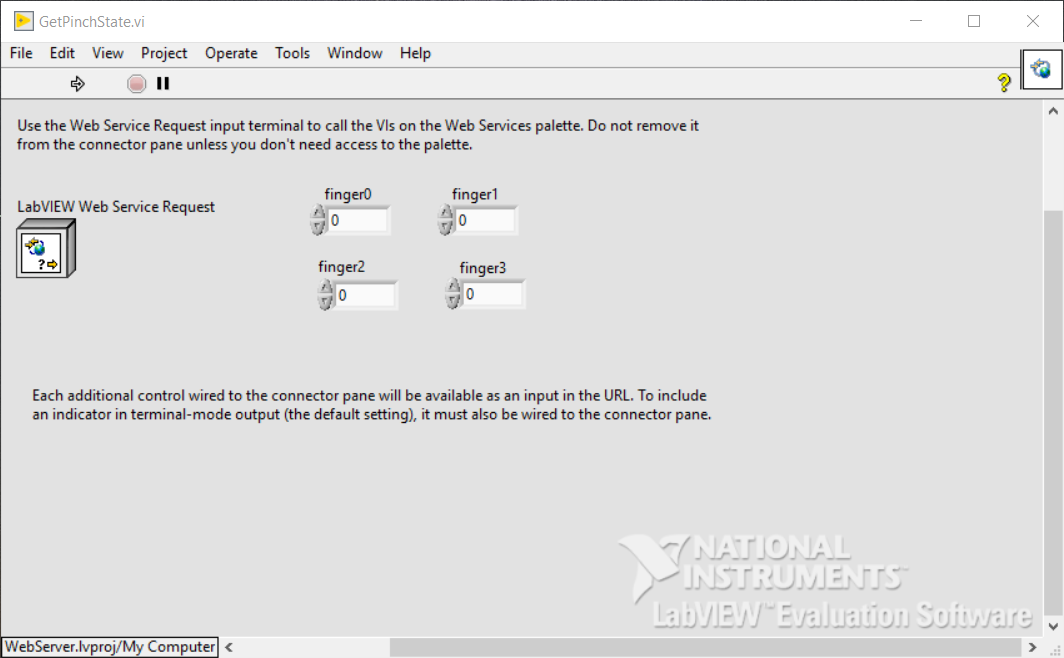
\includegraphics[width=10cm]{Bilder/UserPanel.png}
		\caption{Aufbau des User Panels in der GET-Methode des LabVIEW Servers}
		\label{fig:LabVIEWuserPanel}
	\end{center}
\end{figure}  
In dem User Panel ist der Block LabVIEW Web Service Request angelegt über diesen kommt der GET Request in LabVIEW an.
Des Weiteren sind für jeden der vier gemessenen Finger ein Numeric Control Panel angelegt. Diese sollen den aktuellen Stand der Finger anzeigen.
\begin{figure}[H]
	\begin{center}
		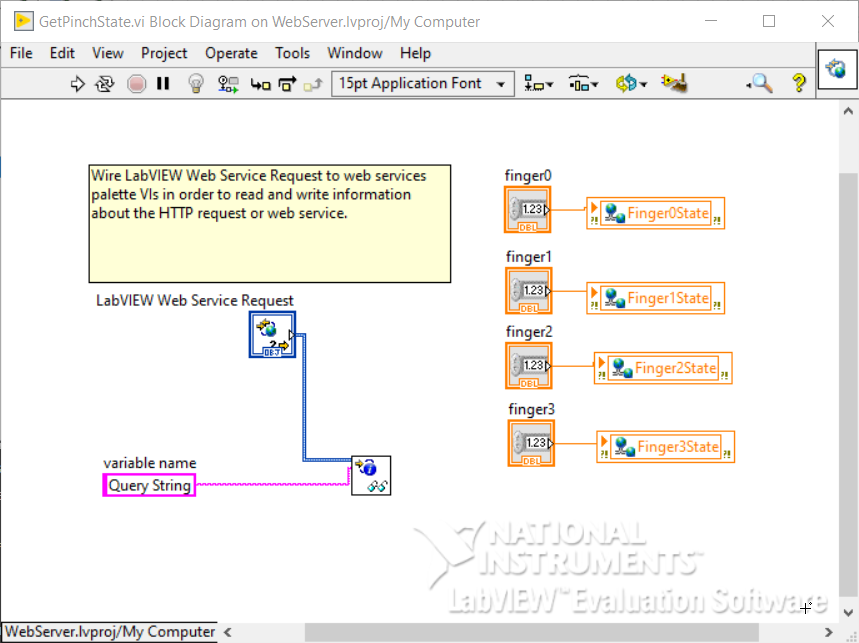
\includegraphics[width=10cm]{Bilder/BlockDiagram.png}
		\caption{Aufbau des Block Diagrams in der GET-Methode des LabVIEW Servers}
		\label{fig:LabVIEWBlockDia}
	\end{center}
\end{figure}
Die beschrieben Blöcke im User Panel werden im Block Diagram miteinander logisch verbunden.
Der Block LabVIEW Web Service Request und ein Query String sind mit dem eigentlichen Server verbunden. Die einzelnen Finger müssen nicht mit dem Server verbunden werden, sie erhalten Ihre Daten durch die Verknüpfung im Connector Pane.
Damit die Werte der Finger außerhalb des Servers verwendet werden können, sind diese mit einer Shared Variable Node verbunden. Somit wird der jeweilige Wert in die globale Variable übernommen und kann von der Ansteuerung der Roboterhand genutzt werden.  
\begin{figure}[H]
	\begin{center}
		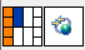
\includegraphics[width=5cm]{Bilder/ConnectorPane.png}
		\caption{Aufbau des Connector Panes in der GET-Methode des LabVIEW Servers}
		\label{fig:LabVIEWConnectorPane}
	\end{center}
\end{figure}  
Im Connector Pane sind von oben nach unten die Finger 0 bis 3 als Input verknüpft (Abbildung \ref{fig:LabVIEWConnectorPane}, orange) und der LabVIEW Web Service Request (blau). 
Dadurch gelangen die Werte an die richtigen Variablen.\\
Mit einem Rechtsklick auf den WebServerHand im Explorer (Abbildung \ref{fig:ProjektExplorer}) kann der Server gestartet werden. Vorher sollten allerdings diese Einstellungen in der NI-Webserver-Konfiguration vorgenommen werden (Abbildung \ref{fig:EinstellungenWebServer}).
\begin{figure}[H]
	\begin{center}
		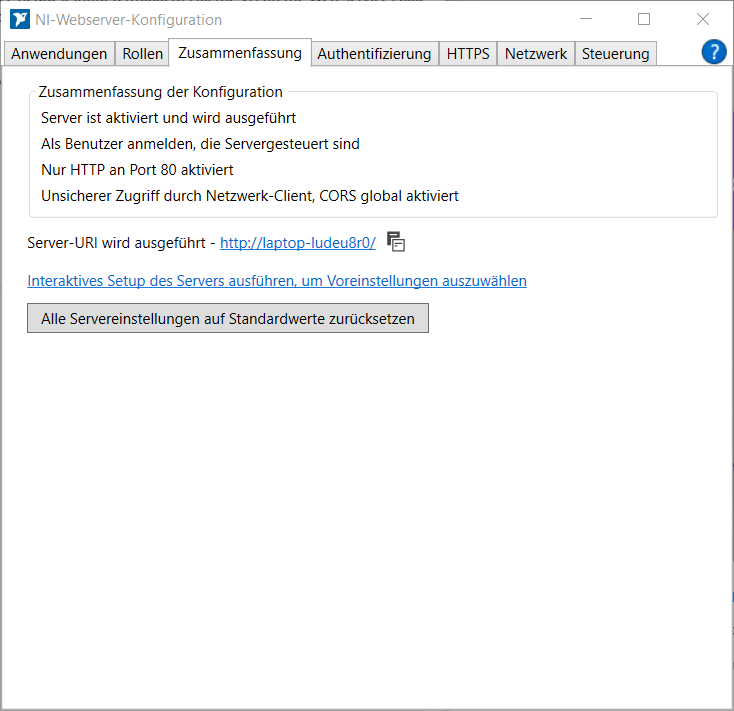
\includegraphics[width=8cm]{Bilder/Einstellungen-StartServerNeu.png}
		\caption{Nötige Einstellungen in der NI-Webserver-Konfiguration}
		\label{fig:EinstellungenWebServer}
	\end{center}
\end{figure}
Sind diese Einstellungen vorgenommen und der Server gestartet, so kann über einen Rechtsklick auf die GetPinchState.vi (Abbildung \ref{fig:ProjektExplorer}) die Methoden-URL angezeigt werden (Abbildung \ref{fig:HTTPMethod})
\begin{figure}[H]
	\begin{center}
		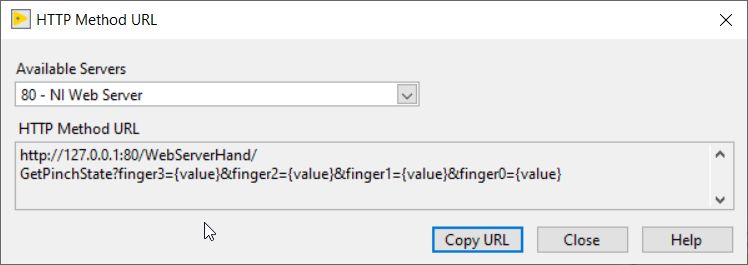
\includegraphics[width=12cm]{Bilder/HTTPMethod.png}
		\caption{URL des HTTP-GET Servers}
		\label{fig:HTTPMethod}
	\end{center}
\end{figure}
Zur Nutzung des Webservers muss Lediglich diese URL in einen Browser eingefügt werden und \glqq \{value\}\grqq\ durch einen Wert ersetzt werden.
Anstelle der angegeben IP-Adresse kann auch \glqq localhost\grqq angegeben werde wenn der Browser und der Server sich auf dem selben PC befinden.
Möchte man den Server auf einem anderen PC laufen lassen, so muss die IP-Adresse durch die des PC's im Netzwerk ersetzt werden.
\subsection{Demonstration}
In dem angehängtem Video (Anhang 3, DemoVideo.mkv), ist auf der linken Seite das User Panel des LabVIEW Webserver zu sehen und auf der rechten Seite die Weboberfläche (Abbildung \ref{fig:ScreenshotVideo}).
\begin{figure}[H]
	\begin{center}
		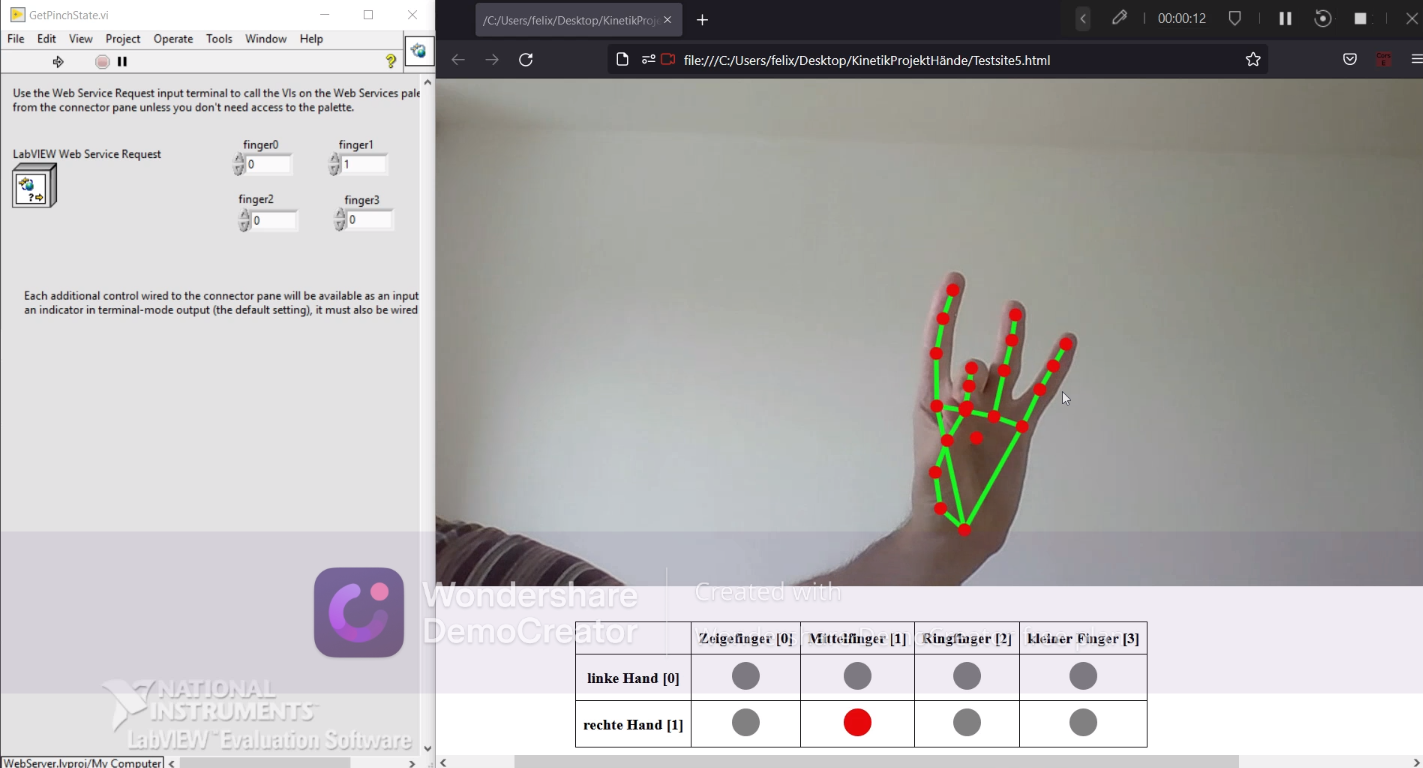
\includegraphics[width=12cm]{Bilder/ScreenshotVideo.png}
		\caption{Screenshot aus dem Demovideo im Anhang}
		\label{fig:ScreenshotVideo}
	\end{center}
\end{figure}
Es ist im Videofeed rechts zu erkennen das sich der Mittelfinger und der Daumen berühren. In der Tabelle darunter sieht man das in der Weboberfläche erkannt wurde, dass sich nur diese Finger berühren.
In dem User Panel links ist zu sehen, dass lediglich bei Finger 1 der Wert von 0 auf 1 geändert wurde. Die Berührung wurde also korrekt erkannt und an LabVIEW übermittelt.\\
Das Demonstrationsvideo lässt den Prozess etwas langsam und verzögert wirken. Dies liegt allerdings nur daran das der Testrechner mit einer schwachen und über 10 Jahren alten CPU ausgestattet ist und gleichzeitig den Bildschirm aufzeichnet. 
Ohne Bild\-schirm\-auf\-zeich\-nung läuft der Prozess flüssig und deutlich schneller. 
\newpage
\section{Fazit}
\emph{Diskussion (Interpretation und Beurteilung der Ergebnisse)}
\newpage
\section{Ausblick}
\emph{Zusammenfassung und Ausblick (Vorschläge für weiterführende Arbeiten)}
Mehr Hände\\
genaueres Tracking (werte von bis)
\newpage
\pagenumbering{Alph}
\phantomsection 
\addcontentsline{toc}{section}{Literaturverzeichnis} %Fügt das Literaturverzn soeichnis zum Inhaltsverzeichnis hinzu
\printbibliography  % Literaturliste ausgeben.
\newpage
\section*{Anhang} \sectionmark{Anhang}
\addcontentsline{toc}{section}{Anhang} %Fügt den Anhang zum Inhaltsverzeichnis hinzu
\begin{enumerate}
	\item Code für die Website \_\_\_.html
	\item Code des LabVIEW-Projektes \_\_\_
	\item Demonstrations Video DemoVideo.mkv
\end{enumerate}
\newpage

\end{document}